\section{Solving Laplace's Equation in Two Dimensions}
\label{sec:laplace}

Here Laplace's equation in two dimensions,
\begin{equation}
    \nabla^2 \varphi = 0,
\end{equation}
is solved using the finite difference equation given in Equation \ref{eqn:iteration} with $\rho = 0$. The chosen convergence condition is that the maximum change in any node is less than an absolute error tolerance, called $\epsilon$. By default $\epsilon$ is set to $10^{-5}$, but choosing a different scale for the charge density requires altering this to be appropriate, e.g. if the charges involved are $\mathcal{O}(10^{-6})$, the absolute error tolerance should be $\sim 10^{-11}$.\todo{I might change this.} All non-boundary nodes were set to random guesses between 0 and 1. The number of iterations was capped at \texttt{max\_it}$=10000$.

\subsection{Basic Verification}
\label{subsec:basic_verification}

The program has in-built boundary conditions for a parallel plate capacitor, a plane equipotential, a single point charge-like equipotential in the middle of the grid, a net with constant potential around the edges of the grid and a cross equipotential. The resulting solutions are plotted in Figures \ref{fig:basic_examples}.

\begin{figure}
    \centering
    \subfloat[Contour plot]{
        \includegraphics[width=0.3\linewidth]{graphs/examples/plane_contour.eps}
        \label{subfig:plane_cont}
    }
    \subfloat[Surface plot]{
        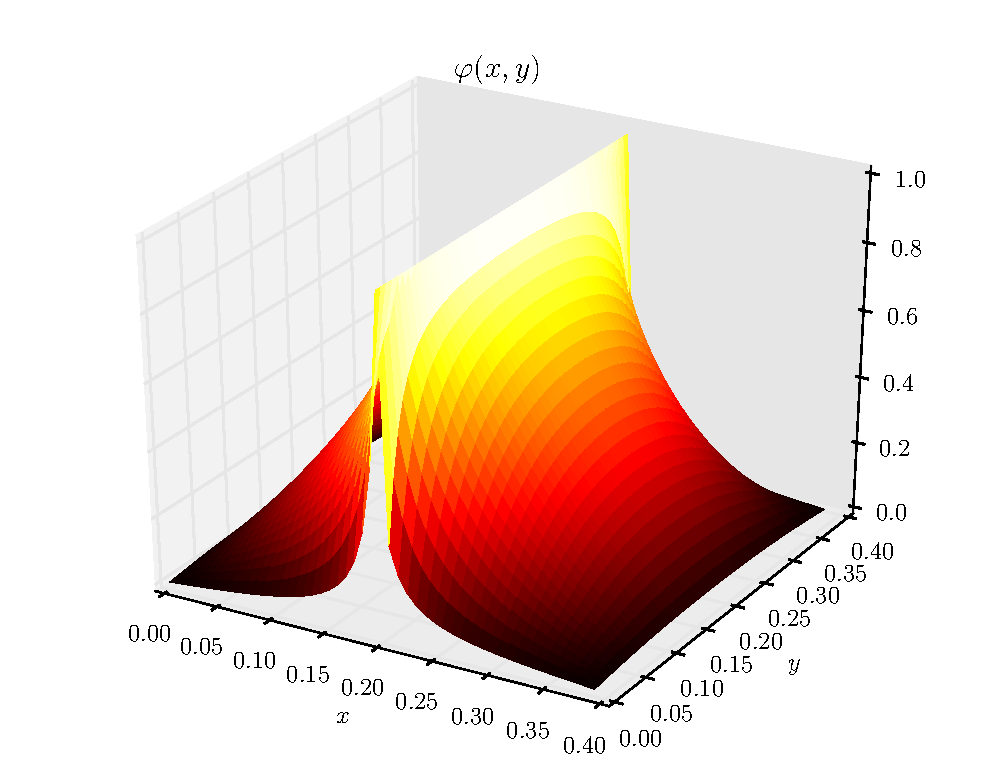
\includegraphics[width=0.3\linewidth]{graphs/examples/plane_surf.eps}
        \label{subfig:plane_surf}
    }
    \subfloat[Vector \textbf{E} field plot]{
        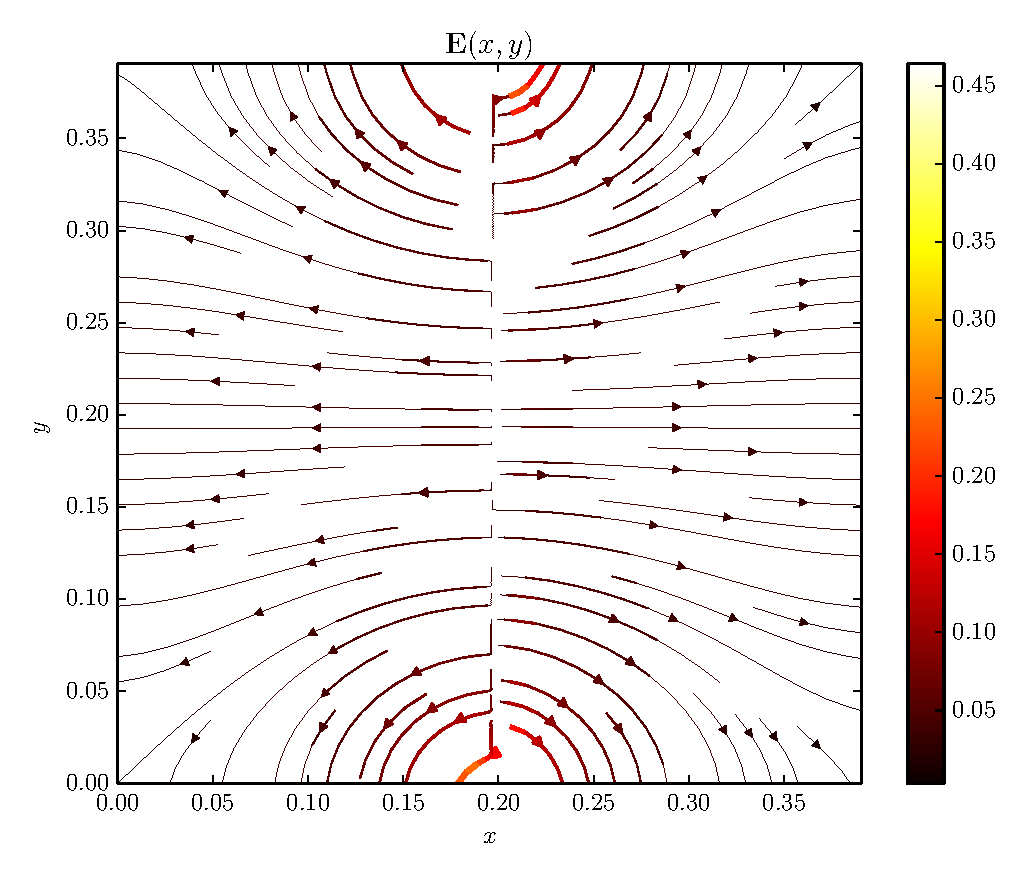
\includegraphics[width=0.3\linewidth]{graphs/examples/plane_vector.eps}
        \label{subfig:plane_vect}
    }
    \caption{Plots of the solution to the Laplace equation with boundary conditions of an equipotential plane.}
    \label{fig:plane}
\end{figure}

\begin{figure}
    \centering
    \subfloat[Contour plot]{
        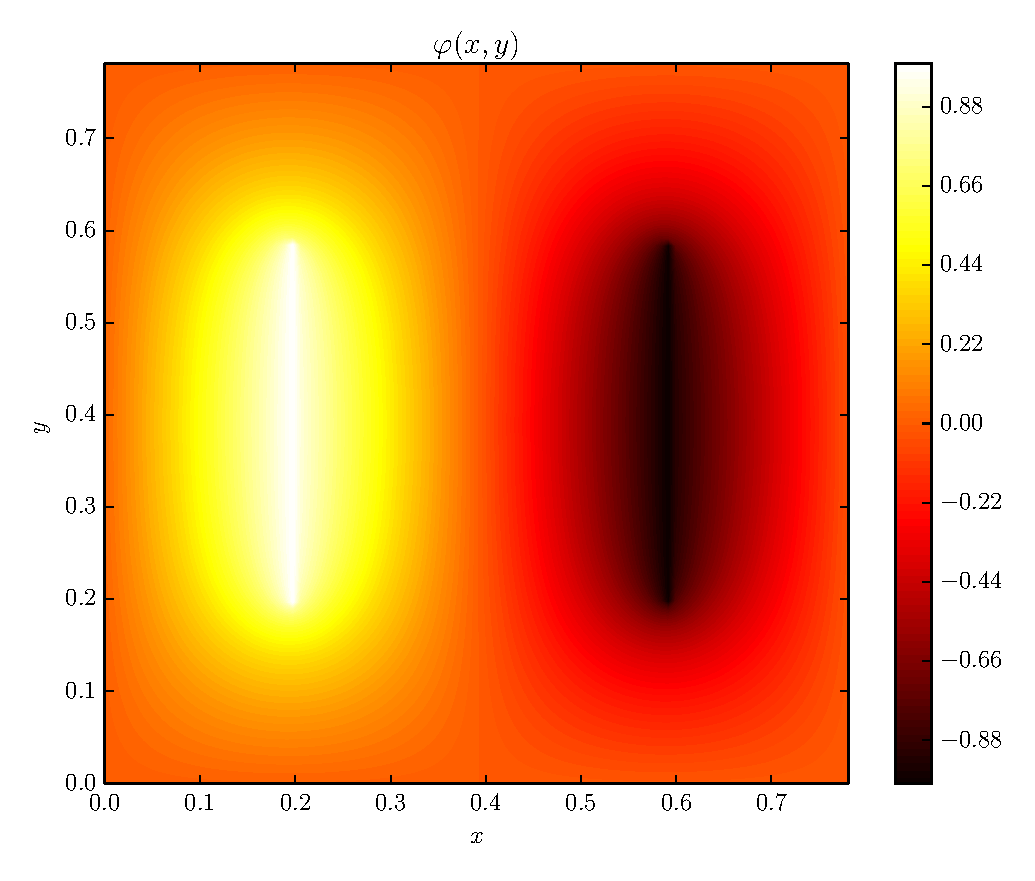
\includegraphics[width=0.3\linewidth]{graphs/examples/capacitor_contour.eps}
        \label{subfig:capacitor_cont}
    }
    \subfloat[Surface plot]{
        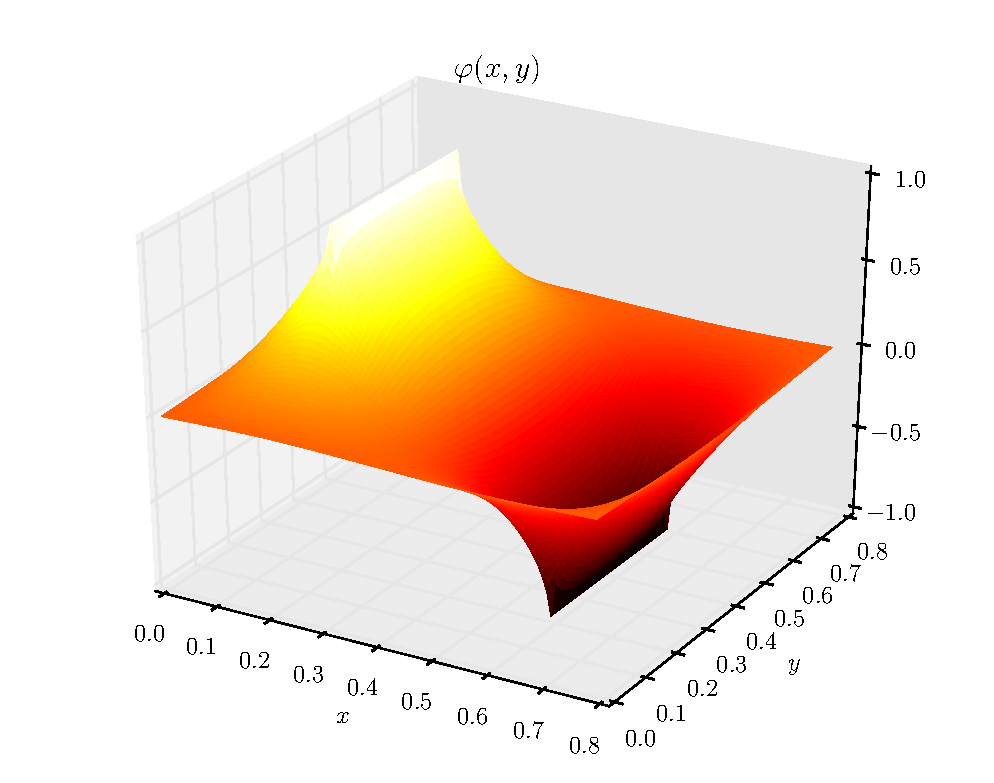
\includegraphics[width=0.3\linewidth]{graphs/examples/capacitor_surf.eps}
        \label{subfig:capacitor_surf}
    }
    \subfloat[Vector \textbf{E} field plot]{
        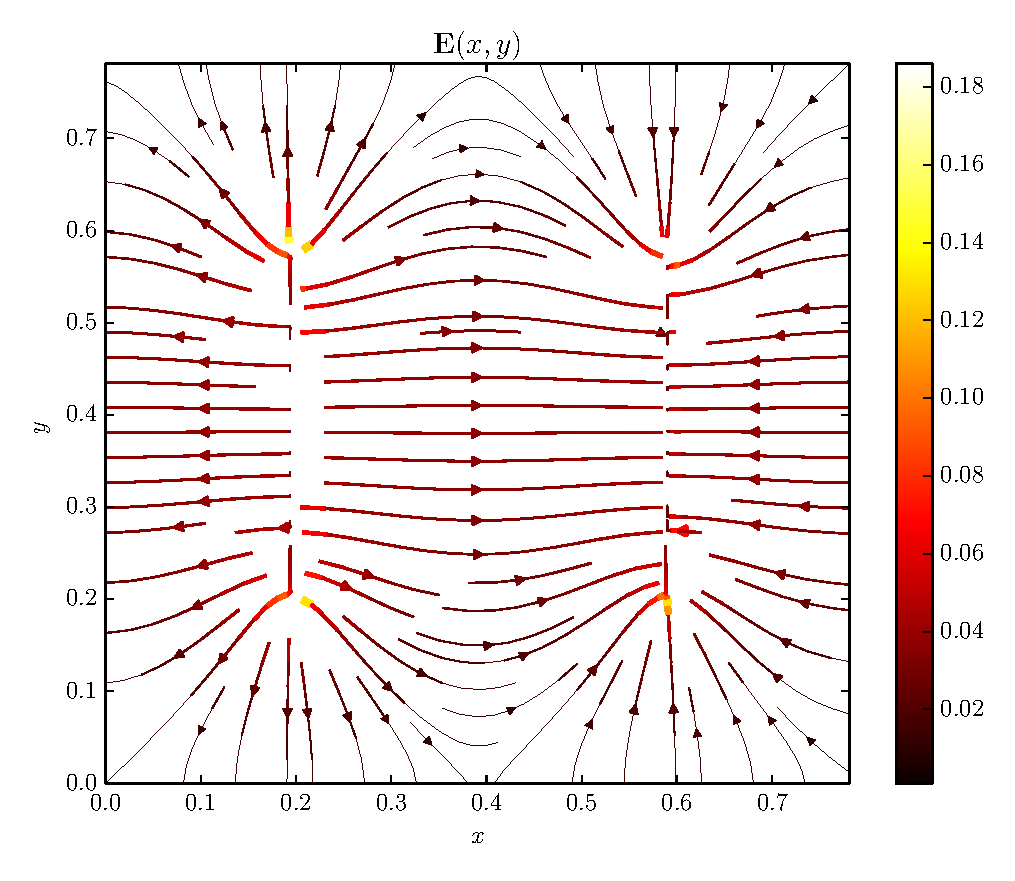
\includegraphics[width=0.3\linewidth]{graphs/examples/capacitor_vector.eps}
        \label{subfig:capacitor_vect}
    }
    \caption{Plots of the solution to the Laplace equation for a parallel plate capacitor.}
    \label{fig:plane}
\end{figure}

\begin{figure}
    \centering
    \subfloat[Contour plot]{
        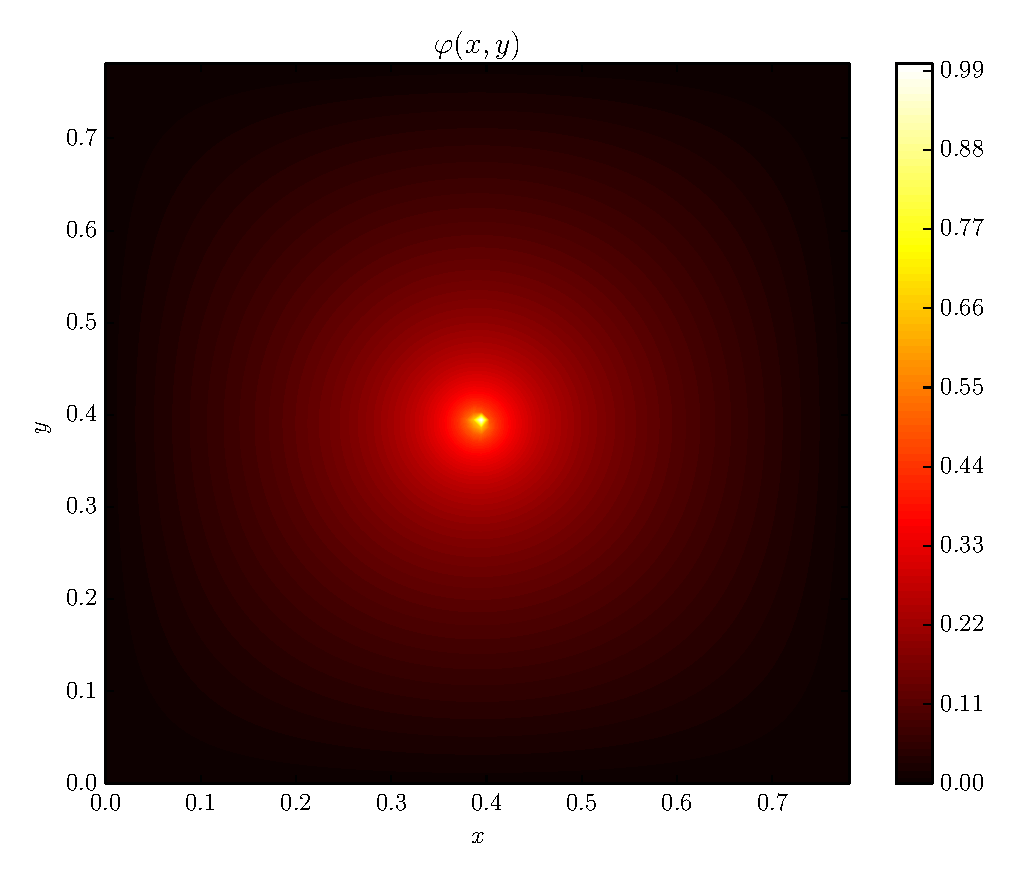
\includegraphics[width=0.3\linewidth]{graphs/examples/point_charge_contour.eps}
        \label{subfig:point_charge_cont}
    }
    \subfloat[Surface plot]{
        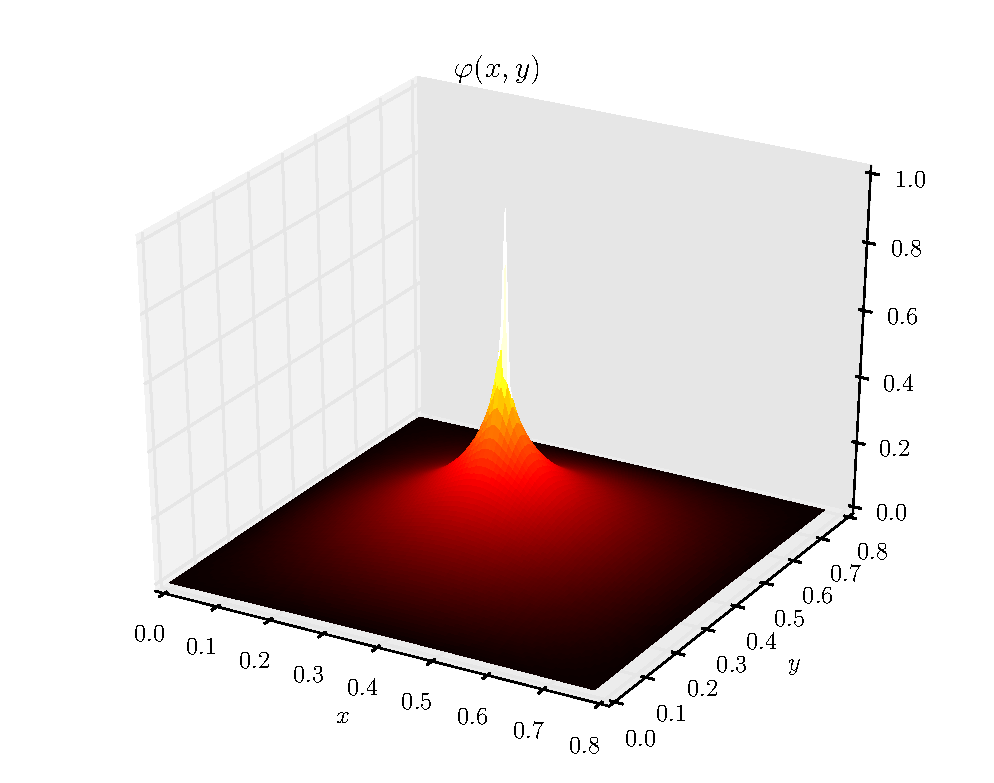
\includegraphics[width=0.3\linewidth]{graphs/examples/point_charge_surf.eps}
        \label{subfig:point_charge_surf}
    }
    \subfloat[Vector \textbf{E} field plot]{
        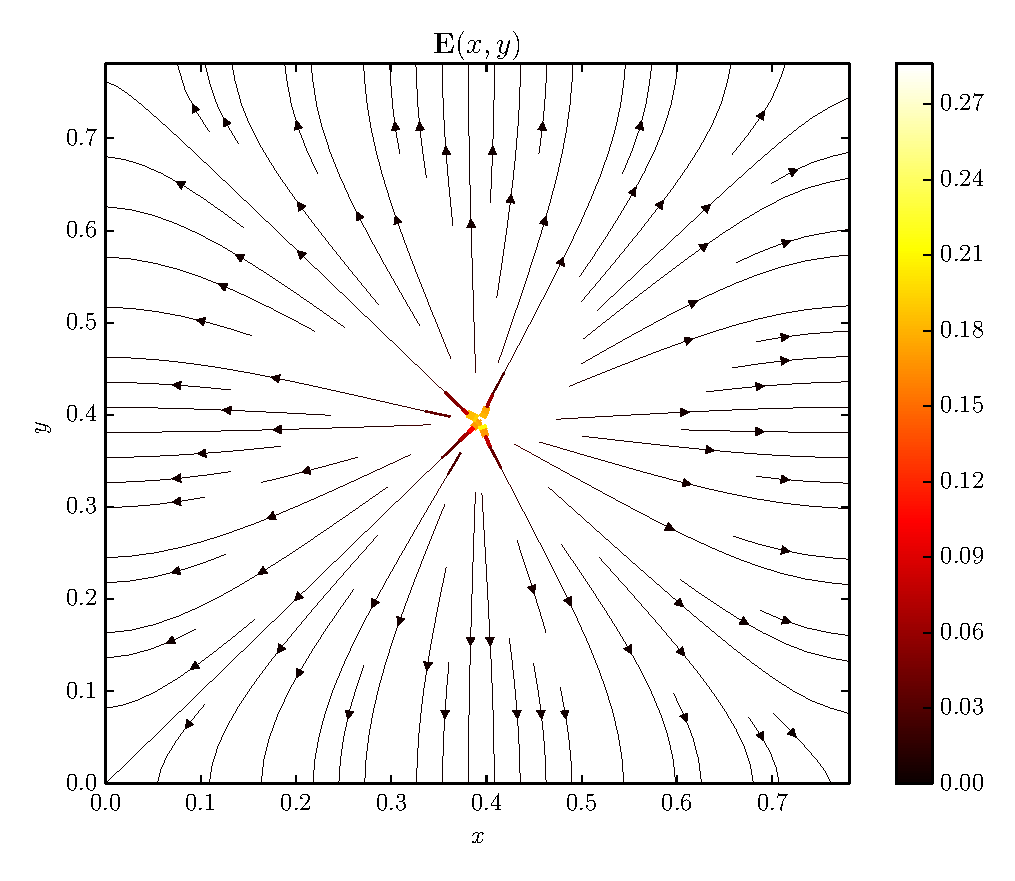
\includegraphics[width=0.3\linewidth]{graphs/examples/point_charge_vector.eps}
        \label{subfig:point_charge_vect}
    }
    \caption{Plots of the solution to the Laplace equation for a single constant potential point.}
    \label{fig:plane}
\end{figure}

\begin{figure}
    \centering
    \subfloat[Contour plot]{
        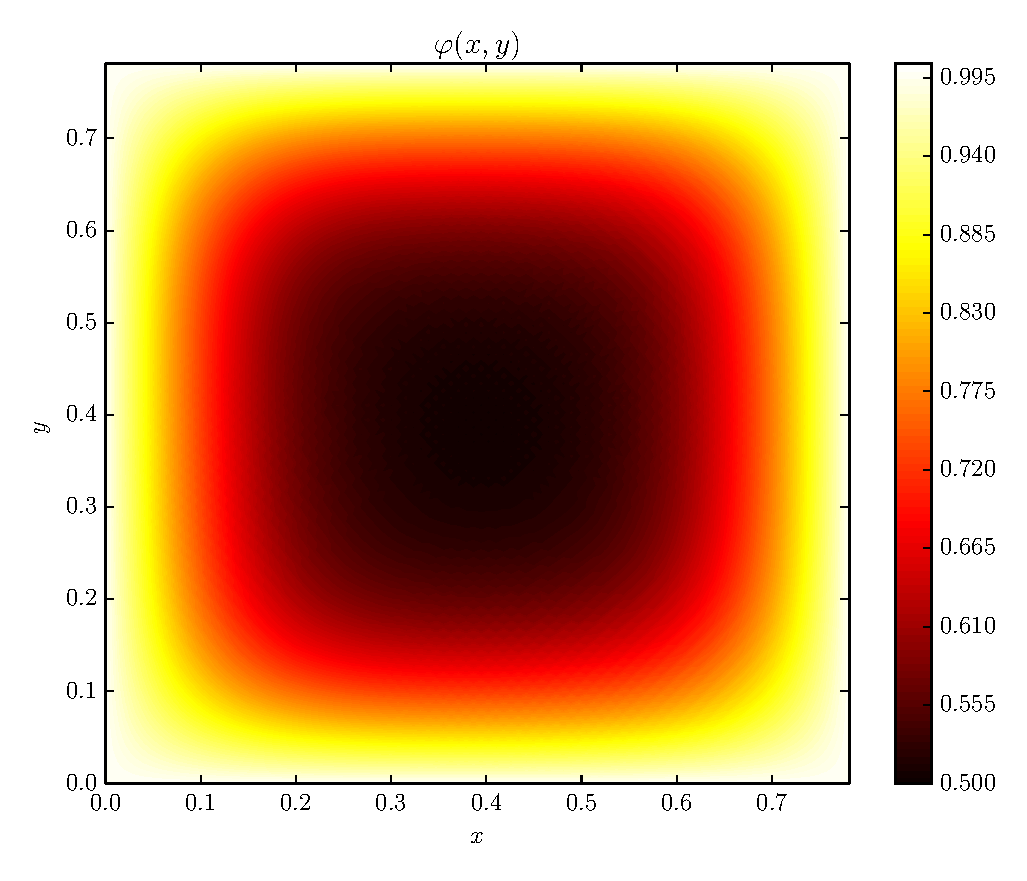
\includegraphics[width=0.3\linewidth]{graphs/examples/net_contour.eps}
        \label{subfig:net_cont}
    }
    \subfloat[Surface plot]{
        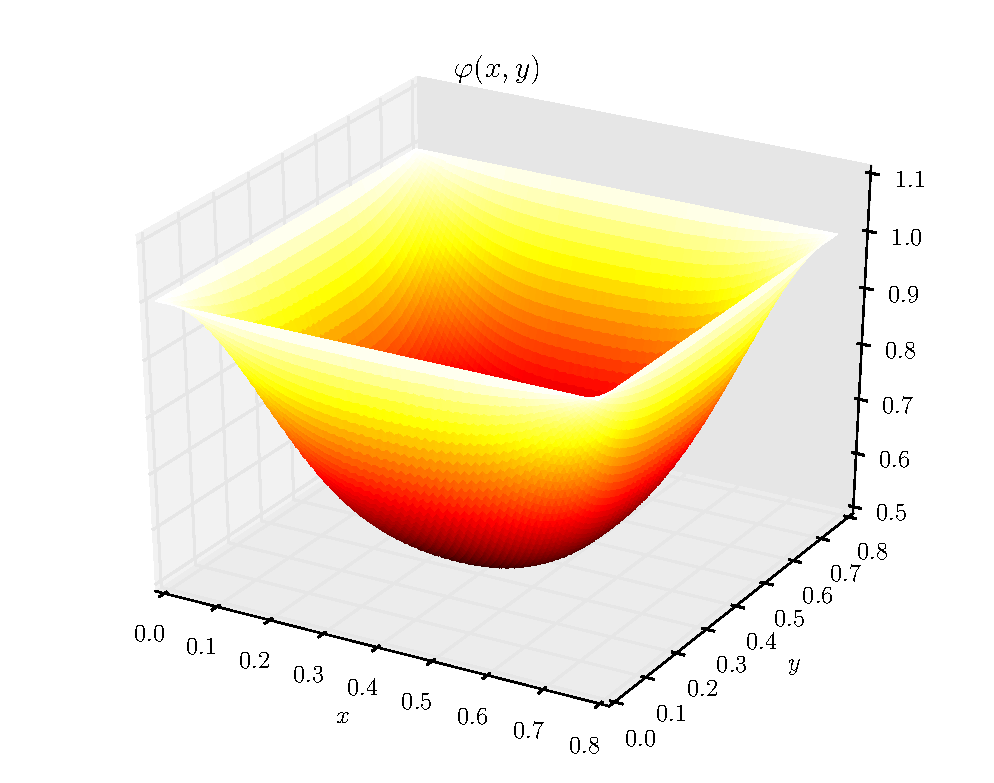
\includegraphics[width=0.3\linewidth]{graphs/examples/net_surf.eps}
        \label{subfig:net_surf}
    }
    \subfloat[Vector \textbf{E} field plot]{
        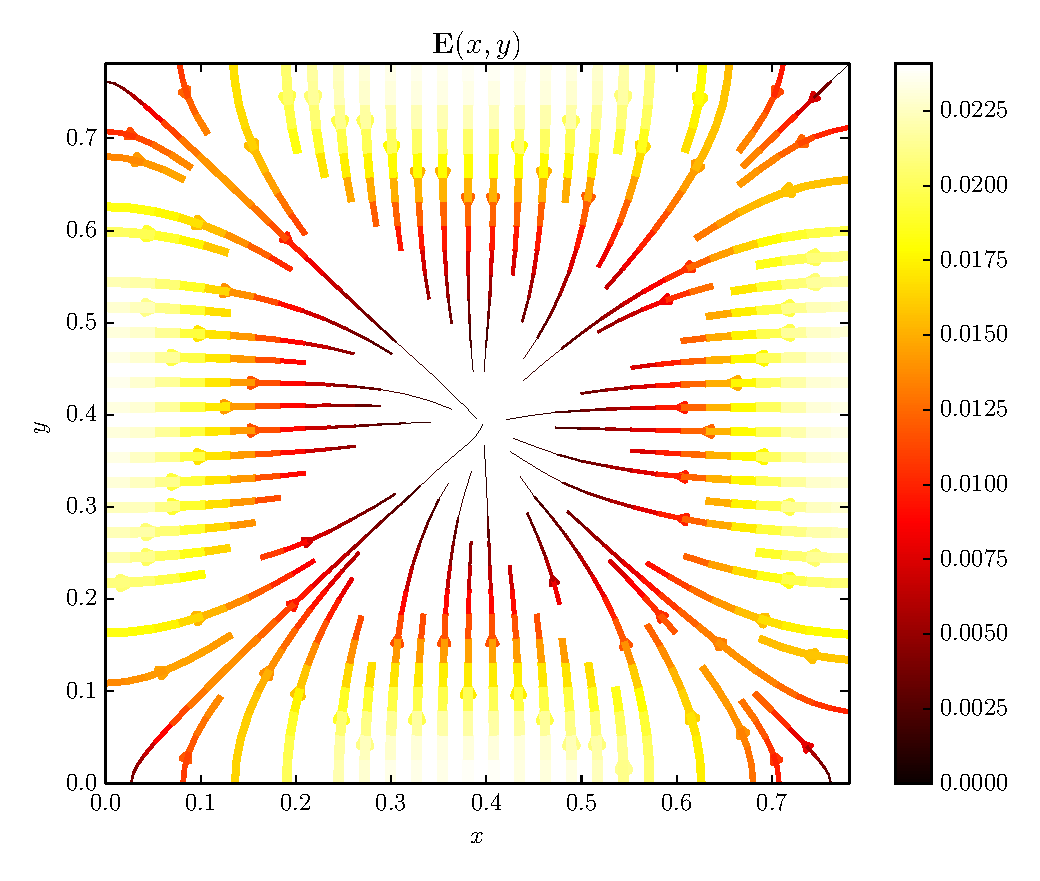
\includegraphics[width=0.3\linewidth]{graphs/examples/net_vector.eps}
        \label{subfig:net_vect}
    }
    \caption{Solution to the Laplace equation with edges of the grid held at constant positive potential.}
    \label{fig:plane}
\end{figure}

\begin{figure}
    \centering
    \subfloat[Contour plot]{
        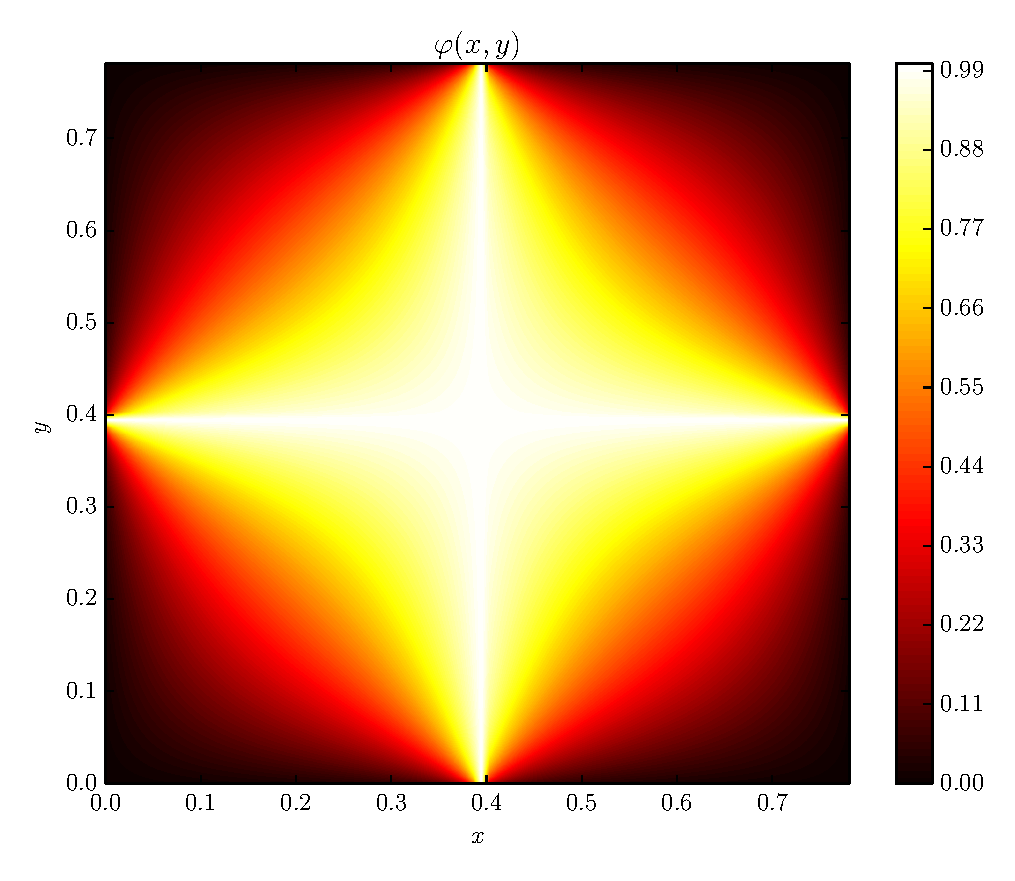
\includegraphics[width=0.3\linewidth]{graphs/examples/cross_contour.eps}
        \label{subfig:cross_cont}
    }
    \subfloat[Surface plot]{
        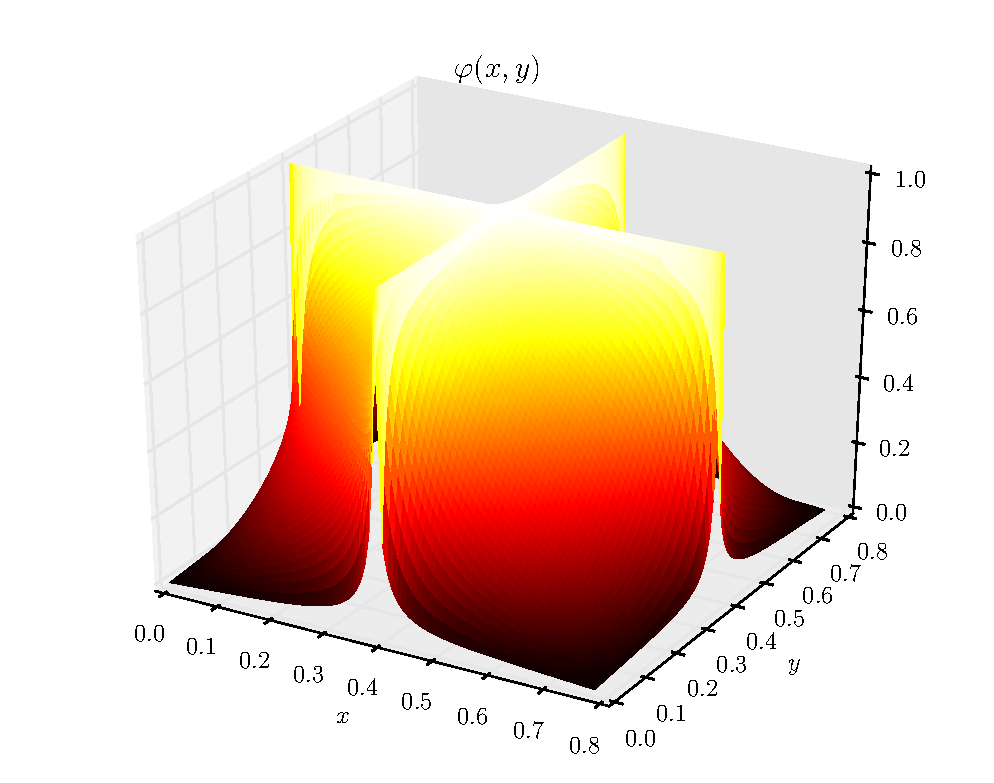
\includegraphics[width=0.3\linewidth]{graphs/examples/cross_surf.eps}
        \label{subfig:cross_surf}
    }
    \subfloat[Vector \textbf{E} field plot]{
        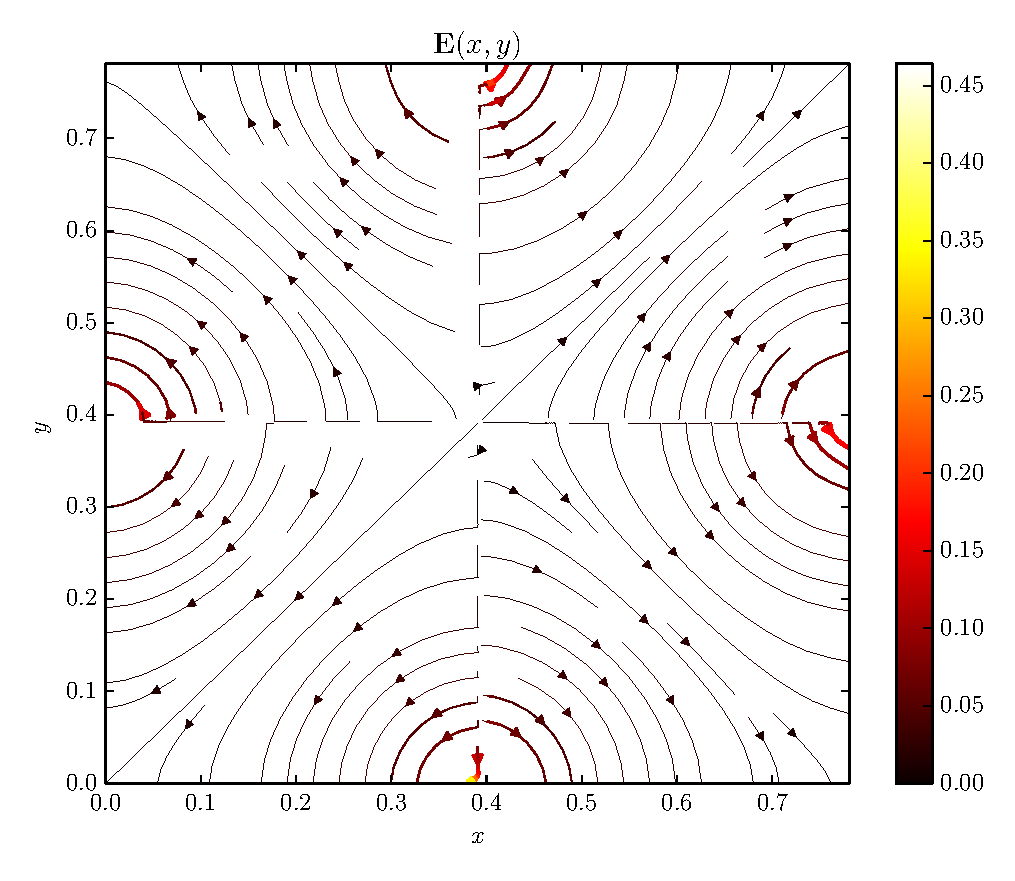
\includegraphics[width=0.3\linewidth]{graphs/examples/cross_vector.eps}
        \label{subfig:cross_vect}
    }
    \caption{Solution to the Laplace equation with equipotential cross overlaid on grid.}
    \label{fig:plane}
\end{figure}

\subsection{Convergence Condition}
\label{subsec:convergence_condition}

An absolute convergence condition is implemented to decide when the program has successfully iterated to the solution of the Laplace equation with the set boundary conditions. As compared to a relative convergence conditions, e.g. that no value changes by more than $X\%$, this has the disadvantage of depending on the boundary conditions applied to the system. So an absolute error tolerance of $\epsilon = \SI{0.01}{V}$ may be appropriate if the highest boundary condition is $\mathcal{O}(100)\si{V}$, but inappropriate if the potential boundary condition is $\mathcal{O}(0.1)$\si{V}. This is compensated for by the ability to manually change the error tolerance with the \texttt{--error} flag. By default this value is set at $10^{-4}$. When the boundary conditions are a single constant potential of \SI{1}{V} at the centre of the grid, the effect of a relatively large tolerance is to fatten the potential field around the point in the centre, as shown in Figure \ref{fig:tolerances}. This is because a too high $\epsilon$ means the iterations stop before a true solution is found. As there are no charges involved, the effect of each iteration is merely to average from the surrounding nodes. Hence when the program finishes the iterations early, it means it has prematurely ceased this averaging process and thus is higher near the central peak than it should physically be. \todo{Analysis of how changing the convergence condition changes the results out at the end, maybe with particular reference to the point charge which looks a bit squiffy for large tolerance.}

\begin{figure}
    \centering
    \subfloat[$\epsilon = 10^{-2}$]{
        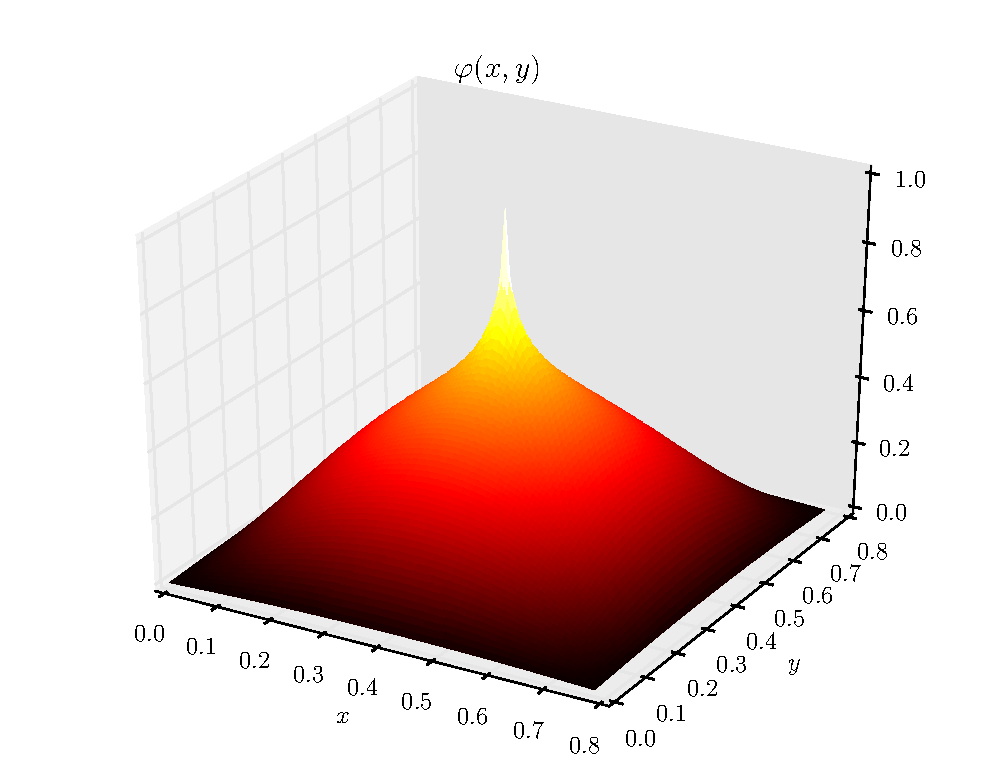
\includegraphics[width=0.5\linewidth]{graphs/tolerance/point_charge_error_1e-2_surf.eps}
        \label{subfig:error_1e-2}
    }
    \subfloat[$\epsilon = 10^{-6}$]{
        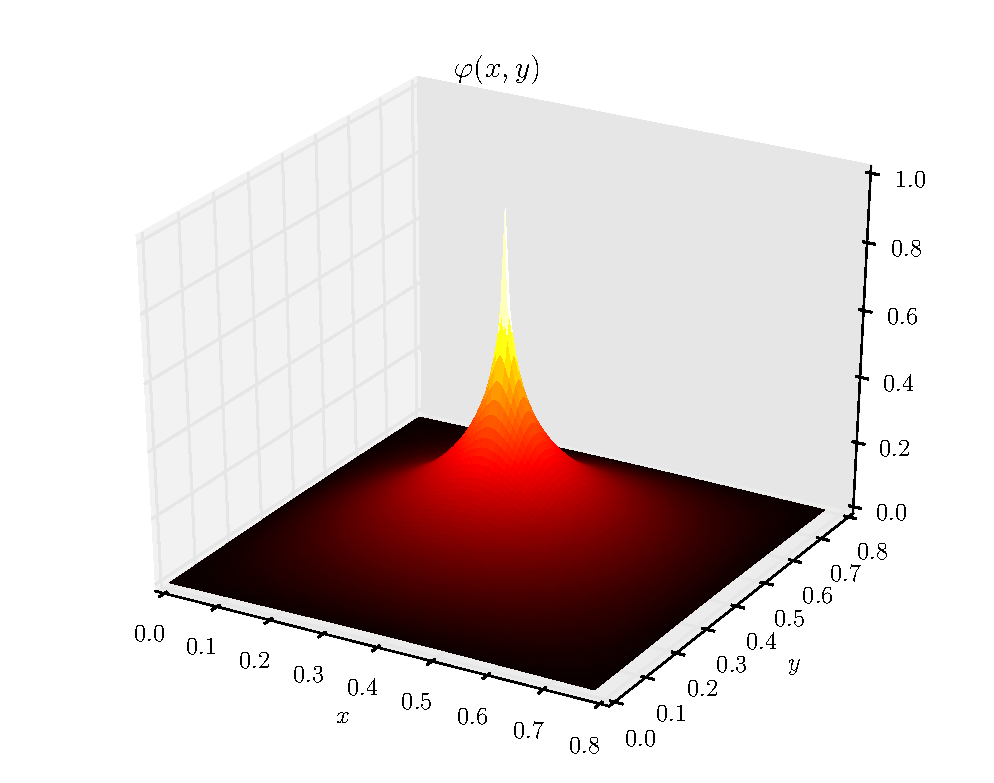
\includegraphics[width=0.5\linewidth]{graphs/tolerance/point_charge_error_1e-6_surf.eps}
        \label{subfig:error_1e-6}
    }
    \caption{Comparison of the effect of altering the absolute error tolerance, $\epsilon$, in the convergence condition on the resulting solution.}
    \label{fig:tolerances}
\end{figure}

\subsection{Iteration Method}
\label{subsec:convergence_condition}

Both the Jacobi and Gauss-Seidel iteration methods are implemented, with the option of which to use left up to the user with the positional argument \texttt{method} determining which to use. It is noticed that the Gauss-Seidel method is significantly faster than the Jacobi, particularly when computing the solution at high grid densities.\todo{A quantitative analysis of the difference in the timing between the two methods, including varying the grid density, with the aim of showing how much faster the Gauss-Seidel implementation is.}\todo{Comparison of consistency of results; include why it doesn't work for the net.}

\subsection{Grid Density}
\label{subsec:grid_density}

The default parameters of the grid density are a 50 by 50 grid. Changing the density significantly affects the time taken to find a converging solution. For the Jacobi method, the time taken to find the solution to the Laplace equation with the boundary conditions of a parallel plate capacitor...\todo{Detailed time analysis, possibly with table.} Combining high density with very low tolerance results in extremely long convergence times, as shown by \todo{Detailed analysis of what happens when you've got both high grid density (100x100) and low tolerance (1e-6).}.

\subsection{Grid Edges}
\label{subsec:grid_edges}

